% !TEX root = thesis.tex
\chapter{Further Out}
\label{chap:furout}

In this chapter we advance the goal of
an $\oout F_n$ analog to
the
Brendle-Margalit Theorem \cite{meta}
by considering subcomplexes of the
sphere complex $\mathcal S_n$
that are themselves combinatorial models.
We will largely argue by extending automorphisms
from subcomplexes of $\mathcal S_n$ to automorphisms
of $\mathcal S_n$ by finding a combinatorial characterization
of any absent type of sphere.

In Section
\ref{sect:sepspheres} we consider the complex of separating spheres.
In Section
\ref{section:highgenussep}
we consider the complex of separating sphere with sufficiently complex sides.
In Section \ref{section:ffc}
we consider the complex of coconnected spheres and its relation to the free factor complex.


\section{Complex of Separating Spheres}
\label{sect:sepspheres}

Let $\mathcal {S}^{sep}_{n,p} \subset \mathcal {S}_{n,p}$ be the complex of embedded homotopy classes of separating spheres
in $M_{n,p}$. In this section we will aim to show that the complex of separating spheres is a combinatorial model for $\oout_{n,p}$.

\thmsepspheres*

We begin by computing the dimension.

\begin{lemma}
\label{sepflagdim}
$\mathcal {S}^{sep}_{n,p}$ is a flag complex of dimension $2n+p-4$.\\
\end{lemma}
\begin{proof}
$\mathcal {S}^{sep}_{n,p}$ is the induced subcomplex of $\mathcal {S}_{n,p}$,
which is known to be flag \cite{souto}.
We show by induction that any collection $\Sigma$ of disjoint spheres
in $M_{n,p}$
is a subset of a
maximal collection of $\max(2n+p-3,0)$ disjoint spheres.

Suppose for a base case that $\Sigma = \varnothing$.
Any pants decomposition of the surface $S_{n,p}=\partial H_{n} - P$ by curves surrounding
disks in the handlebody $H_n$ with punctures $P$ has
$3n-3+p$ curves with $n$ of them nonseparating.
Taking an identical copy of $\partial H_{n}-P$ and gluing along $S_{n,p}$
promotes the pants decomposition of $S_{n,p}$ into a decomposition of $M_{n,p}$ into $M_{0,3}$s.
Of these $3n-3+p$ spheres, $n$ are nonseparating and $2n+p-3$ are separating.

Assume that any collection of $k$ or fewer disjoint spheres in $M_{n,p}$ is a subset of a
maximal collection of $2n+p-3$ disjoint spheres.
Let $\Sigma$ be a collection of $k$ disjoint spheres and let $x$
be a sphere disjoint from all spheres of $\Sigma$.
Then cutting $M_{n,p}$ along $x$ yields two components
homeomorphic to
$M_{n',p'}$ and $M_{n'',p''}$ where $n'+n'' =n$ and $p'+p''=p+2$.
By inductive hypothesis, the set spheres of $\Sigma$ in each component can
extended to maximal sets $\Sigma_1$ and $\Sigma_2$ of size
$2n'+p'-3$
and
$2n''+p''-3$
respectively.
Then $\Sigma \cup \{x\}$ is contained in the maximal set
$\Sigma_1 \cup \Sigma_2 \cup \{x\}$ of size
$$
(2n'+p'-3) + (2n''+p''-3) + 1 =2n+p-3.
$$
\end{proof}


\begin{lemma}
  $\mathcal {S}^{sep}_{n,p}$ is connected
whenever it has positive dimension, except if
$(n,p)=(2,1)$.
\end{lemma}


\begin{proof}
Consider first the case where $n=0$.
There is a deformation retraction of $M_{0,s}$ away from the puncture $p_s$ to a wedge product $\bigvee_{i \in s-1}S^2_i$ of $p-1$ copies of $p^2$.
We thus have $\pi_2(M_{0,s}) \cong \Z^{s-1}$.
If $x$ is an embedded sphere of $M_{0,s}$ separating the set of punctures $\{p_{i_1}, \ldots, p_{i_k}\}$ from the other punctures, then the map
$$
\begin{tikzcd}
x \arrow[hookrightarrow]{r}
& M_{0,s}  \arrow{r}
& \bigvee_{i \in s-1}S^2_i \arrow{r}
 &S^2_{p_k}
\end{tikzcd}
$$
is degree 1 if $x$ separates $p_k$ from $p_s$ and 0 otherwise.
(See degree theory of \cite{MR1867354}.)
So there are $2^{s-1}-1$ homotopy classes of spheres in $M_{0,s}$,
with each sphere totally determined by
its
bipartition of the punctures.
Let $P$ be the punctures.
So $\mathcal {S}^{sep}_{0,s}$ is the
isomorphic to the complex of
bipartitions of $P$ with size
with two bipartitions adjacent if their sides give nested subsets of $P$.
Then
if
$p \geq 5$ there is a path
in $\mathcal {S}^{sep}_{0,s}$ between any two spheres
made by moving elements between the partitions one at a time.


Consider the case where $n \geq 1$.
We make use of Putman's Lemma \ref{lemma:putman}
where $G = \oout_{n,p}$ and $X=\mathcal {S}^{sep}_{n,p}$.
Fix a sphere $v$ that bounds an embedded copy of $M_{1,1}$ in $M_{n,p}$.
Note that $\oout_{n,p}$ acts transitively on
such spheres, and every separating sphere that does not
bound an embedded copy of $M_{1,1}$
is disjoint from such a sphere.
So the orbit $\oout_{n,p} \cdot v$ intersects
the connected component of every separating, considered as a vertex of
$\mathcal {S}^{sep}_{n,p}$.

Consider a free basis $a_1, \ldots, a_n, b_1, \ldots, b_s$
of the free group $F_{n+p}$
with $v$ disjoint from the spheres representing the basis
and $v$ separating $a_1$ from $a_2, \ldots, a_n$.
Take as a generating set of $\oout_{n,p}$
the transpositions of $\{b_1, \ldots, b_s\}$,
the transpositions and inversions of $\{a_1, \ldots, a_s\}$,
the transvection $a_1 \mapsto a_1a_2^{-1}$,
and
the conjugation $b_1 \mapsto a_1b_1a_1^{-1}$.


Observe that transpositions of $\{b_1, \ldots, b_s\}$
and inversions of $\{a_1, \ldots, a_n\}$
leave $v$ fixed.
Further, transpositions of $\{a_1, \ldots, a_n\}$
either fix $a_1$ and thus $v$, or move $v$ to a disjoint separating sphere
at distance 1 from $v$ in $\mathcal {S}^{sep}_{n,p}$.

Consider the image $v'$ of $v$ under the
conjugation $b_1 \mapsto a_1b_1a_1^{-1}$,
as shown in green in Figure \ref{sepconnect}.

\begin{figure}[b!]
    \centering
    \begin{subfigure}[t]{0.3\textwidth}
        \includegraphics[width=\textwidth]{figures/sepconnect0.pdf}
        \caption{The basepoint sphere $v$ separates $a_1$
        from $a_2,\ldots, a_n$ and $b_1, \ldots, b_s$.}
        \label{fig:sepconnect0}
    \end{subfigure}
    ~
    \begin{subfigure}[t]{0.3\textwidth}
        \includegraphics[width=\textwidth]{figures/sepconnect1.pdf}
        \caption{The transvection $a_1 \mapsto a_1a_2^{-1}$
        corresponds to
        pushing $a_1^+$ through $a_2^-$.}
        \label{fig:sepconnect1}
    \end{subfigure}
    ~
    \begin{subfigure}[t]{0.3\textwidth}
        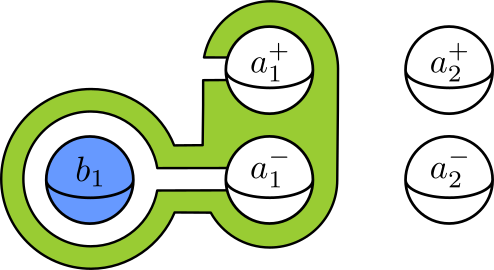
\includegraphics[width=\textwidth]{figures/sepconnect2.pdf}
        \caption{The conjugation $b_1 \mapsto a_1b_1a_1^{-1}$
        corresponds to pushing
        $b_1$ through $a_1^+$.}
        \label{fig:sepconnect2}
    \end{subfigure}
    \caption{Nontrivial $\oout_{n,p}$ generator actions on the base sphere $v$
    move $v$ at most distance 2 in $\mathcal S^{sep}_{n,p}$.}
    \label{sepconnect}
\end{figure}


Then $v'$ and $v$ are contained in a copy of $M_{1,2}$ bounded by $b_1$
and the sphere $u$ separating $a_1$ and $b_1$ from
$a_2, \ldots, a_n$ and $b_2, \ldots, b_s$.
If $n\geq 2$ or $p\geq 3$ we have that $u$
is essential and this gives a length 2 path $v$ to $u$ to $v'$ in $\mathcal {S}^{sep}_{n,p}$.
The inverse conjugation $b_1 \mapsto a_1^{-1}b_1a_1$ similarly
moves $v$ distance 2 in $\mathcal {S}^{sep}_{n,p}$.
Appealing to Putman's Lemma \ref{lemma:putman}, we conclude that
$\mathcal {S}^{sep}_{n,p}$ is connected for $n=1$ and $p\geq 3$.

Suppose $n \geq 2$.
Then generation of $\oout_{n,p}$ also requires transvection.
Consider the image $v'$ of $v$ under the
diffeomorphism corresponding to
the transvection $a_1 \mapsto a_1a_2^{-1}$,
as shown in orange in Figure \ref{sepconnect}.
Then $v'$ and $v$ are contained in a copy of $M_{2,1}$ bounded by
the sphere $u$ separating $a_1$ and $a_2$ from
$a_3, \ldots, a_n$ and $b_1, \ldots, b_s$.
If $n\geq 3$ or $p\geq 2$ we have that $u$
is essential and this gives a length 2 path $v$ to $u$ to $v'$ in $\mathcal {S}^{sep}_{n,p}$.
The inverse transvection $b_1 \mapsto a_1a_2$ similarly
moves $v$ distance 2 in $\mathcal {S}^{sep}_{n,p}$.
Appealing to Putman's Lemma \ref{lemma:putman}, we conclude that
$\mathcal {S}^{sep}_{n,p}$ is connected for $n=2$ and $p\geq 2$ or $n\geq 3$.




Finally, we show that $\mathcal {S}^{sep}_{2,1}$
is disconnected.
By capping the boundary component with a sphere we obtain a map
$$
\phi: \left (\mathcal {S}^{sep}_{2,1} \right )^{(0)} \to \left (\mathcal {S}^{sep}_{2,0} \right )^{(0)}
$$
Observe that if $u$ and $v$ are disjoint spheres of $\mathcal {S}^{sep}_{2,1}$
then $\phi(u)=\phi(v)$.
So $\phi$ gives a surjective simplicial map
$$
\mathcal {S}^{sep}_{2,1}  \to \mathcal {S}^{sep}_{2,0}.
$$
But as $\mathcal {S}^{sep}_{2,0}$ is totally disconnected it must be that ${S}^{sep}_{2,1}$
is disconnected.
\end{proof}


\noindent
We say that a sphere is $M_{n',p'}$-bounding if it bounds an embedded copy of $M_{n',p'} \subset M_{n,p}$.

\begin{lemma}
  \label{sepgenpreserved}
For $k\leq n/2$,
$M_{k,1}$-bounding spheres are characteristic in $\mathcal {S}^{sep}_{n}$ for $n\geq 3$.
\end{lemma}
\begin{proof}
Suppose that $x \in \mathcal {S}^{sep}_{n}$ bounds
an $M_{k,1}$.
Observe the link of $x$ is isomorphic to
a join
$\mathcal S^{sep}_{k,1}  \ast \mathcal S^{sep}_{n-k,1}$.
By Lemma \ref{sepflagdim}
the dimensions of the sides of the join are $2k-3$ and $2n-2k-3$,
so any automorphism of $\mathcal {S}^{sep}_{n}$
must send $x$ to a genus $k$-bounding sphere.
\end{proof}


Observe that
$M_{1,0} = S_1 \times S_2$
so that $\pi_2(M_{1,0},p) \cong \Z$.
Using the long exact sequence of the pair
$(M_{1,1},\partial M_{1,1})$
we compute  $\pi_2(M_{1,0}) \cong \pi_2 (M_{1,1}, S^2 )$,
so $M_{1,1}$
contains a unique homotopy class of nonseparating sphere
generating the second homotopy group.

Then for any automorphism $\phi \in \aaut \left (  \mathcal S^{sep}_{n,p}\right)$
we can extend $\phi$ to a map
$\hat \phi : \mathcal S_{n,p} \to \mathcal S_{n,p}$.
If $x$ is a separating sphere we assign $\hat \phi (x) = \phi(x)$.
If $a$ is a nonseparating sphere, then
there is there is an $M_{1,1}$-bounding sphere $x$
bounding an $M_{1,1}$ that contains $a$.
Then $\phi(x)$ bounds an $M_{1,1}$ by
Lemma \ref{sepgenpreserved}.
We define $\hat \phi(a)$ to be
the nonseparating sphere in the $M_{1,1}$ bounded by $\phi(x)$.
We must first demonstrate that $\hat \phi$ is well defined.

Fix a nonseparating sphere $a$.
Define a \emph{sharing pair} $\{x,x'\}$ (sharing $a$) to be
$M_{1,1}$-bounding spheres $x$ and $x'$
such that $x$ and $x'$ each bound an $M_{1,1}$ containing $a$
and are contained in a common $M_{2,1}$ bounded by separating sphere $y$.

\begin{lemma}
  \label{sepsharepair}
If $\{x,x'\}$ is a sharing pair, then $\{\phi(x),\phi(x')\}$
is a sharing pair for any
automorphism $\phi \in \aaut\left( \mathcal S^{sep}_{n} \right )$.
\end{lemma}

\begin{proof}
Let $a_1$ be a nonseparating sphere of $M_{n,p}$
and let $\{x,x'\}$ be a sharing pair for $a_1$.
Then $x$ and $x'$ are adjacent to an $M_{2,1}$-bounding sphere $y$,
but not each other in $\mathcal S^{sep}_{n}$.
Let $a_2$ be a nonseparating sphere disjoint from $a_1$ in the $M_{2,1}$ bounded by $y$.
Observe further we may find an $M_{1,1}$-bounding sphere
$z$ that intersects $y$, but not $x$ or $x'$.
\begin{figure}
% \floatbox[{\capbeside\thisfloatsetup{capbesideposition={right,top},capbesidewidth=.4\textwidth}}]{figure}[\FBwidth]
% {
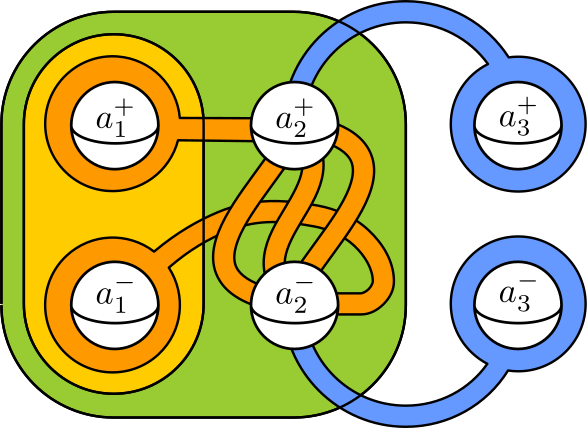
\includegraphics[width=.6\textwidth]{figures/sepsharepair.pdf}
\caption{
The sharing pair $x$ and $x'$ bound $M_{1,1}$ shown in yellow and orange.
They are contained in the green $M_{2,1}$ bounded by $y$.
The blue $M_{1,1}$ is bounded by $z$.
Observe an $M_{1,1}$-bounding sphere containing $a_1$ can be represented
by drawing two parallel copies $a^+_1$ and $a^-_1$ and then connecting them
by attaching a handle given by the regular neighborhood of an arc from $a_1^-$ to $a^+_1$ disjoint from $a_1$.
Fixing $a_1$, the spheres $x$ and $x'$ are determined by their respective intersection numbers with $a_2$.
}
\label{sepshare}
\end{figure}
Then, appealing to Lemma \ref{sepsharepair}, $\phi(x)$ and $\phi(x')$
must be intersecting $M_{1,1}$-bounding spheres.
Let $A$ be the $M_{2,1}$ bounded by $\phi(y)$.
$\phi(z)$ is disjoint from $\phi(x)$ and $\phi(x')$, but not $\phi(y)$.
Consider the image of $\phi(z)$ in the $A$.
If $\phi(z)$ bounded a region containing a nonseparating sphere in
$A$, there would only be one class of separating sphere in $A$
disjoint from $\phi(z)$.
Then $\phi(z)$  must bound in $A$
a handle given by the boundary of a regular neighborhood of an arc of
$\pi_1(A,\partial A)$ that must pass through a nonseparating sphere $a$ of $A$.
But then $\phi(x)$ and $\phi(x')$ must both bound the nonseparating sphere of $A$ disjoint from $a$.
So $\{\phi(x),\phi(x')\}$ is a sharing pair.
\end{proof}

Let $a$ be a nonseparating sphere of $M_n$.
We will show that any two $M_{1,1}$-bounding spheres
that contain $a$ on their $M_{1,1}$-side are connected by a sequence of
sharing pairs.
Let $\mathcal P_a$ be the \emph{sharing pair} graph defined as follows.
The vertices of $\mathcal P_a$
are genus 1-bounding separating spheres of $M_n$ that
bound an $M_{1,1}$ containing $a$.
Two vertices of $\mathcal P_a$ are adjacent
if they form a sharing pair for $a$.

\begin{lemma}
  \label{seppairgraph}
The sharing pair graph $\mathcal P_a$ is connected.
\end{lemma}

\begin{proof}
We appeal to Putman's Lemma \ref{lemma:putman}
using the graph $X=\mathcal P_a$ and the group
$G \leq \oout_{n}$ fixing $a$ setwise.
Let $a_1, \ldots, a_n$ be a basis for $F_n$.
Then $G$ is generated by
diffeomorphisms corresponding to
permutations of $\{a_2, \ldots, a_n\}$,
inversions, and the transvections
$a_1 \mapsto a_1a^{-1}_2$ and $a_2 \mapsto a_2a^{-1}_3$.

Observe that $G$ acts transitively on
$M_{1,1}$-bounding spheres
that contain $a$ on their genus 1-side.
Let $v$ be the sphere separating
$a_1$ from $a_2, \ldots, a_n$.
Observe that of the chosen generators only
the transvection $\phi: a_1 \mapsto a_1a^{-1}_2$
has nontrivial action on $v$.
But, as can be seen in figure \ref{sepconnect},
 $v$ and $\phi(v)$
 are contained in an $M_{2,1}$
 so that  $\{ v, \phi(v) \}$ is a sharing pair.

 It follow by Putman's Lemma \ref{lemma:putman} that $\mathcal P_a$ is connected.
\end{proof}

The previous Lemma shows that $\hat \phi$ is well defined.
If $a$ is a nonseparating sphere of $M_n$
and $x$ and $x'$ $M_{1,1}$-bounding sphere bounding an $M_{1,1}$ containing $a$,
then as $P_a$ is connected there is a sequence of sharing pairs from $x$ to $x'$.
By Lemma \ref{sepsharepair} this gives a sequence of
sharing pairs from $\phi(x)$ to $\phi(x')$.
But then $\phi(x)$ and $\phi(x')$ share the same nonseparating sphere
so that $\hat \phi (a)$ is well defined.

Certainly $\hat \phi$ is simplicial.
If $a$ and $a'$ are disjoint nonseparating spheres
then there are disjoint $M_{1,1}$-bounding spheres $x$ and $x'$ bounding
disjoint copies of $M_{1,1}$ separating $a$ and $a'$, respectively.
Since $\phi(x)$ and $\phi(x')$ are disjoint $M_{1,1}$-bounding spheres,
$\hat \phi(a)$ and $\hat \phi(a')$ are also disjoint.
If $y$ is a separating sphere disjoint from $a$, then
either there is an $M_{1,1}$-bounding sphere separating $a$ from $y$
or $y$ is an $M_{1,1}$-bounding sphere, so that $\hat \phi(a)$ is disjoint from $\hat \phi (y) = \phi(y)$.


% \thmsepspheres*

\begin{proof}[Proof of Theorem \ref{thm:sep}.]
The map constructed above
$$\Phi: \aaut \left ( \mathcal S^{sep}_n \right) \to \aaut \left ( \mathcal S_n \right)$$
with $\phi \mapsto \hat \phi$
is an isomorphism with the  map simply restricting automorphisms
$$\aaut \left ( \mathcal S_n \right) \to   \aaut \left ( \mathcal S^{sep}_n \right)$$
giving an inverse to $\Phi$.
Then the result follows from
Theorem \ref{aramsouto}.
\end{proof}

\section{Complexes of High Genus Separating Spheres}
\label{section:highgenussep}

For $k\leq n/2$, we call a sphere $x: S^2 \hookrightarrow M_{n,p}$ $k$-separating
if both components of
$M_{n,p}-x$
contain either a boundary component
or at least $k$ disjoint separating spheres.
If $x$ bounds a copy of $M_{j,1}$ with $j<n/2$,
we refer to it as to as $x^{in}$, or the \emph{inside} of $x$.
We will also describe objects disjoint from and inside of $x$ as \emph{engulfed} by $x$,
and disjoint objects on the outside as \emph{exgulfed} by $x$.

Let $\mathcal S^{sep,k}_{n,p} \subset \mathcal S^{sep}_{n,p}$
be the subcomplex spanned by homotopy classes of essential $k$-separating
spheres.
In this section we show that $\mathcal S^{sep,k}_{n,p}$ is a combinatorial model for $\oout_{n,p}$.

\thmhighsep*

Observe that for $k>1$,
$\mathcal S^{sep,k}_{n,p}$
does not have a uniform dimension.
For example, in the case with no boundary components, $p=0$,
we can construct
a maximal (with respect to inclusion)
simplex of maximal dimension
\hbox{$n-2k$}
as in Figure \ref{bigsimp}.
\begin{figure}[b!]
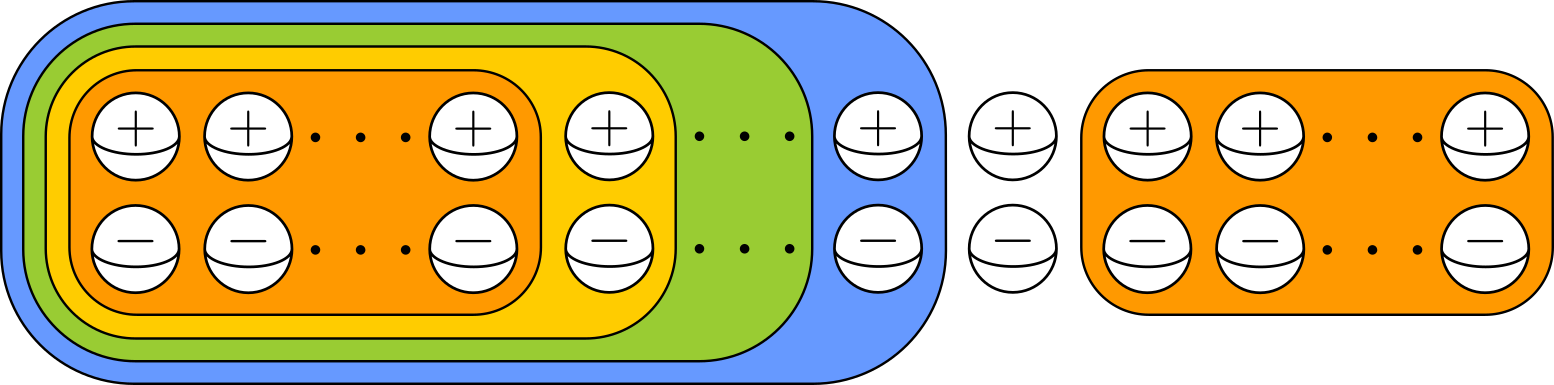
\includegraphics[width=\textwidth]{figures/bigsimplex.pdf}
\caption{A maximal dimension maximal simplex of $\mathcal S^{sep,k}_{n}$ for $k>1$
is spanned by $n-2k+1$ spheres and cuts $M_n$ into 2 copies of $M_{k,1}$ and $n-2k$
copies of $M_{1,2}$.
The corresponding graph of $M_{n}$ components is an unbranched tree
with 2 leaves of weight $k$ and $n-2k$ internal vertices of weight 1.}
\label{bigsimp}
\end{figure}
If we write $n=qk+r$ with $q = \lfloor n/k \rfloor$ and $0<r<k$,
then we can construct maximal (with respect to inclusion) simplices
of smaller dimension $2q+r-4$ as in Figure \ref{lilsimp}.
\begin{figure}[b!]
\includegraphics[width=\textwidth]{figures/smallersimplex.pdf}
\caption{A minimal dimension maximal simplex of $\mathcal S^{sep,k}_{n}$ for $k>1$
is spanned by $2q+r-3$ spheres and cuts $M_n$
into $q$ copies of $M_{k,1}$ and $r$ copies of $M_{1,2}$ and $q-2$ copies of $M_{0,3}$.
The corresponding graph of $M_{n}$ components is a tree
with $q$ leaves of weight $k$ and $q-2$ internal vertices weight 0
and $r$ internal vertices of weight 1.}
\label{lilsimp}
\end{figure}

If there are boundary spheres we can construct a maximal dimension simplex
similar to Figure \ref{bigsimp}
by replacing the $M_{k,1}$-bounding spheres with boundary spheres.
Similar linear nesting shows any $k$-separating sphere can be contained in a maximum dimension simplex
of dimension for $k>1$
$$
\max_n \left \{
\Delta^n \hookrightarrow
\mathcal S^{sep,k}_{n,p}
\right \}
=
\begin{cases}
  n-2k & \mbox{ if } p=0\\
  n-k & \mbox{ if } p=1\\
  n+p-3 & \mbox{ if } s\geq 2
\end{cases}.
$$

\begin{lemma}
  \label{ksepconnect}
For $1<k<n/2$,
the complex of $k$-separating spheres
$\mathcal S^{sep,k}_{n,p}$
is connected whenever it has positive dimensional simplices if $p=0$,
and whenever it has 2 dimensional simplices if $p>0$.
\end{lemma}

\begin{proof}
The proof is by Putman's Lemma \ref{lemma:putman}
with the group $\oout_{n,p}$.

Consider first the case with $p=0$
and suppose that $\mathcal S^{sep,k}_{n,p}$ has positive dimensional simplices.
So $n>2k$, and in particular
there are $M_{k,1}$ and $M_{k+1,1}$-bounding spheres in $\mathcal S^{sep,k}_{n,p}$.
Choose a sphere $v$ to be an $M_{k,1}$-bounding sphere.
Observe that every $k$-separating sphere is disjoint from a
$M_{k,1}$-bounding sphere, and the $M_{k,1}$-bounding spheres
are exactly the $\oout_{n}$ orbit of $v$.
Let $a_1,\ldots,a_n$ be a maximal collection of disjoint nonseparating spheres
of $M_{n}$ with $a_1,\ldots, a_k$ engulfed by $v$.
Consider as a generating set for $\oout_{n}$
the transpositions and inversions of $a_1,\ldots,a_n$
and the transposition diffeomorphism $t$ corresponding to $a_1 \mapsto a_1a_{k+1}^{-1}$.
Observe that every inversion fixes $v$.
Observe that a transposition $\phi$ either fixes $v$, in the case it swaps
spheres on the same side of $M_n-v$, or $\phi(v)$ and $v$ are contained in a common
$M_{k+1,1}$-bounding sphere that is $k$-separating, as in Figure
\ref{fig:kput0}.
Finally, $v$ and $t(v)$ are contained in a common
$M_{k+1,1}$-bounding sphere as in Figure \ref{fig:kput1}.
The connectivity then follows by Putnam's Lemma.
\begin{figure}[b!]
    \centering
    \begin{subfigure}[b]{0.4\textwidth}
        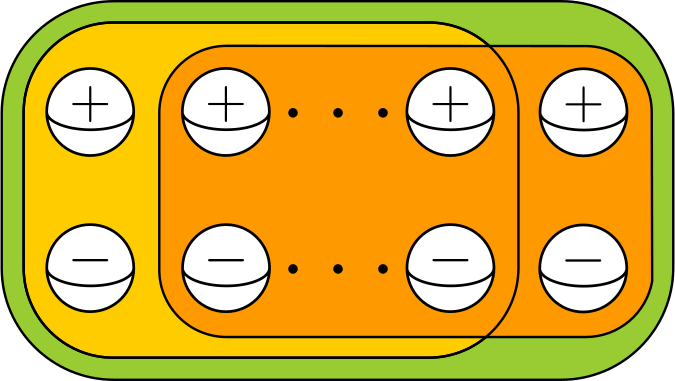
\includegraphics[width=\textwidth]{figures/kput0.pdf}
        \caption{Transpositions move $M_{k,1}$-bounding spheres distance 2.}
        \label{fig:kput0}
    \end{subfigure}
    ~
    \begin{subfigure}[b]{0.4\textwidth}
        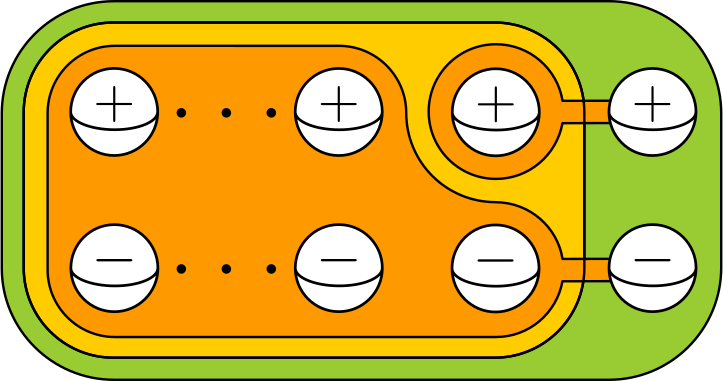
\includegraphics[width=\textwidth]{figures/kput1.pdf}
        \caption{Transvections move $M_{k,1}$-bounding spheres distance 2.}
        \label{fig:kput1}
    \end{subfigure}
    \caption{Nontrivial $\oout_{n}$ generator actions on the base sphere $v$
    move $v$ at most distance 2 in $\mathcal S^{sep,k}_{n,p}$.}
    \label{fig:kput01}
\end{figure}

Consider the case with $p>0$.
If
$p=1$
then to have dimension 2 simplices $n \geq k+2$,
and $M_{2,2}$-bounding spheres are $k$-separating.
If
$p>1$
then to have dimension 2 simplices $n+p\geq 5$.
If $p=1$ then $n \geq 4$
so that $M_{2,2}$-bounding spheres are disjoint from a
$M_{k,1}$-bounding sphere and must be $k$-separating.
If $p>1$ then $n \geq 4$
so that $M_{1,3}$ and $M_{2,2}$-bounding spheres are disjoint from a
$M_{1,2}$ or $M_{k,1}$-bounding sphere and must be $k$-separating.


Choose a sphere $v$ to be an $M_{1,2}$-bounding sphere.
Observe that every $k$-separating sphere is disjoint from a
$M_{1,2}$-bounding sphere, and the $M_{1,2}$-bounding spheres
are exactly the $\oout_{n,p}$ orbit of $v$.
Let $b_1,\ldots,b_s$ be the bounding spheres
and let $a_1$ be a nonseparating sphere engulfed by $v$ and $a_2, \ldots, a_n$
disjoint nonseparating spheres disjoint from $v$ and $a_1$.
Consider as a generating set for $\oout_{n,p}$
diffeomorphisms corresponding to
transpositions of $a_1,\ldots,a_n$,
transpositions of $b_1,\ldots,b_s$,
$t$ the transvection $a_1 \mapsto a_1a_2^{-1}$,
and $u$ the $b_1$ push corresponding to
conjugation $b_1 \mapsto a_1b_1a_1^{-1}$.
Observe first that $u$ leaves $v$ fixed.
Observe  that $\phi$ a
transposition of  $a_1,\ldots,a_n$
either leaves $v$ if it fixes $a_1$, or
swaps $a_1$, and then $\phi(v)$ and $v$
are engulfed by an $M_{2,2}$-bounding sphere as in Figure \ref{fig:kput2}.
Observe that $\psi$ a
transposition of  $b_1,\ldots,b_s$
either leaves $v$ if it fixes $b_1$, or
swaps $b_1$, and then $\psi(v)$ and $v$
are engulfed by an $M_{1,3}$-bounding sphere as in Figure \ref{fig:kput3}.
Finally,
$v$ and $t(v)$
are engulfed by an $M_{2,2}$-bounding sphere as in Figure \ref{fig:kput4}.
The connectivity then follows by Putnam's Lemma.
\begin{figure}[b!]
    \centering
    \begin{subfigure}[b]{0.3\textwidth}
        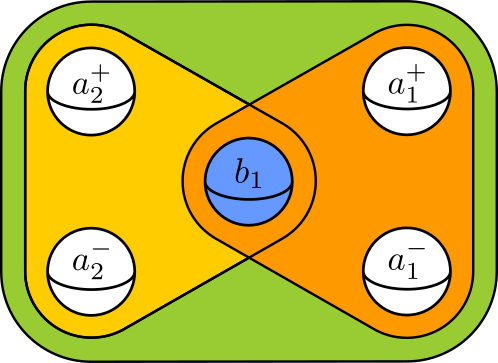
\includegraphics[width=\textwidth]{figures/kput2.pdf}
        \caption{$a$-Transposition}
        \label{fig:kput2}
    \end{subfigure}
    ~
    \begin{subfigure}[b]{0.3\textwidth}
        \includegraphics[width=\textwidth]{figures/kput3.pdf}
        \caption{$b$-Transposition}
        \label{fig:kput3}
    \end{subfigure}
    ~ %add desired spacing between images, e. g. ~, \quad, \qquad, \hfill etc.
      %(or a blank line to force the subfigure onto a new line)
    \begin{subfigure}[b]{0.3\textwidth}
        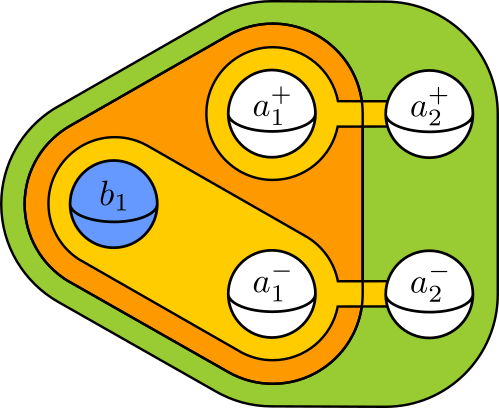
\includegraphics[width=\textwidth]{figures/kput4.pdf}
        \caption{Transvection}
        \label{fig:kput4}
    \end{subfigure}
    \caption{Nontrivial $\oout_{n,p}$ generator actions on the
    base sphere $v$ move $v$ at most distance 2
    in $\mathcal S^{sep,k}_{n,p}$.}
    \label{fig:kput234}
\end{figure}
\end{proof}

\begin{lemma}
Let $n\geq 3$ and $\phi \in \aaut{ \left ( \mathcal S^{sep,k}_{n} \right ) }$.
For $n/2>j\geq k$,
if $x$ is a
$M_{j,1}$-bounding spheres
engulfing a sphere $y$,
then $\phi(x)$
is a
$M_{j,1}$-bounding spheres
engulfing the sphere $\phi(y)$.
\label{kengulfschar}
\end{lemma}

\begin{proof}
  Suppose that $x$ bounds an $M_{j,1}$ in $\mathcal S^{sep,k}_{n}$.
  Consider the subcomplex
  $\mathcal E_x$ spanned by spheres engulfed by $x$
  and the subcomplex
  $\mathcal F_x$ spanned by spheres disjoint but not engulfed by $x$.
  The link of $x$ is a join $\mathcal E_x \ast \mathcal F_x$
  and
  $\mathcal E_x \cong \mathcal S^{sep,k}_{j,1}$
  and $\mathcal F_x \cong \mathcal S^{sep,k}_{n-j,1}$.
  Then according to Lemma \ref{ksepconnect},
  $\mathcal E_x$
  and $\mathcal F_x$
  have simplices with maximal dimension
  $j-k$ and $n-j-k$, respectively.
  So the link of $\phi(x)$ must have the same structure
  and $\phi(x)$ must be $M_{j,1}$-bounding.
  Note that since
  $$\phi \left( \mathcal E_x \right) =\mathcal E_{\phi(x)}$$
  any sphere $y$ engulfed by $x$ has $\phi(y)$ engulfed by $\phi(x)$.
\end{proof}

We hope to extend automorphisms of
$\mathcal S^{sep,k}_{n}$ to
automorphisms of $\mathcal S^{sep,k-1}_{n}$
by
a
combinatorial characterization of
$M_{k-1,1}$-bounding spheres in $\mathcal S^{sep,k}_{n}$.

This is the direct analog of handle pairs of Brendle-Margalit \cite{meta}.

\begin{definition}
  If $x$ is an $M_{k,1}$-bounding sphere engulfed by $M_{k+1,1}$-bounding sphere $y$
  we say that a pair $v,w$ of $M_{k,1}$-bounding spheres
  \emph{carve} $x$ from $y$ if
  \begin{enumerate}[(1)]
    \item Each pair of $v,w,y$ intersects, but $v,w,y$ are all disjoint from $x$.
    $$
    \begin{tikzcd}[every arrow/.append style={dash}]
      v \arrow{r} & x \arrow{r} & y\\
      w \arrow{ur} &&
    \end{tikzcd}
    $$
    \item The $M_{k,1}$-bounding sphere $x$ is the unique sphere engulfed by $y$
    and disjoint from both $v$ and $w$.
    \item There is more than one $M_{k,1}$-bounding sphere engulfed by $y$ and disjoint
    from $v$ but not $w$.
    \item There is more than one $M_{k,1}$-bounding sphere engulfed by $y$ and disjoint
    from $w$ but not $v$.
  \end{enumerate}
\end{definition}

It follows immediately from this combinatorial definition and
Lemma \ref{kengulfschar} that carving is characteristic.
The following Lemma shows additionally that there is
a unique nonseparating sphere that was
``carved away'' from $y$.


\begin{lemma}
  Let $\phi \in \aaut \mathcal S^{sep,k}_{n}$.
  If $v,w$ carve $x$ from $y$,
  then
  \begin{enumerate}[(1)]
  \item $\phi(v), \phi(w)$ carve $\phi(x)$ from $\phi(y)$
  \item One of the spheres $v$ or $w$
  contains a disk or annulus $p$ with $\partial s \subset y$ whose image in $y^{in}/y$
  is homotopic to a nonseparating sphere.
  \item There is an arc $\alpha$ with endpoints on $y$
  such that $v$ and $w$ separate $\alpha$ from $x$.
  \item $x$ is the unique $M_{k,1}$-bounding sphere engulfed by $y$ and disjoint from $p$ and $\alpha$.
\end{enumerate}
\label{carvingchar}
\end{lemma}

\begin{proof}
  (1) follows from Lemma \ref{kengulfschar} and the combinatorial definition of carving.\\
  (2) Fix representatives for $v$, $w$, $x$, and $y$ that intersect minimally and transversely.
  Then $w\cap y^{in}$ is a collection of disks and annuli with boundary on $y$.
  No component disk or annulus of $w\cap y^{in}$ can be separating,
  or else there would be at most $M_{k,1}$ in $y^{in}$
  disjoint from $w$.
  Similarly $v\cap y^{in}$ is a collection of disks and annuli, no one of that separates $y^{in}$.
  Let $\beta$ be any nontrivial loop in $y^{in}-x^{in}$ and based at
  a point on $x$.
  Then $\beta$ must intersect either $v$ or $w$, or else
  the pushes of any nonseparating sphere of $x$ about $\alpha$
  would yield infinitely many $M_{k,1}$-bounding spheres engulfed by $y$
  and disjoint from $v$ and $w$, contrary to the hypothesis.
  Since no such $\beta$ exists,
  there must a component $p$ of $v\cap y^{in}$ or $w\cap y^{in}$
  whose image in the quotient
  $y^{in}/y$ is homotopic to a nonseparating sphere.\\
  (3) Let $a$ be a nonseparating sphere engulfed by $y$ and exgulfed by $x$
  and disjoint from the nonseparating component $p$ as above.
  If $v\cap y^{in}$ or $w\cap y^{in}$
  have a component that intersects $a$, then as $v$ and $w$ are separating there
  must be an arc intersecting $a$ with endpoints on $y$ that they separate from $x$.
  Suppose that $v$ and $w$ are disjoint from $a$.
  If there is a loop $\gamma$ based at $a$ that winds through a noseparating sphere engulfed by $x$
  and is disjoint from $v$ and $w$,
  then the pushes of $a$ along $\gamma$ leave $v$ and $w$ unchanged,
  but the images of $x$ give infintely many $M_{k,1}$-bounding spheres
  engulfed by $y$ and disjoint from $v$ and $w$, in contradiction
  with the definiton of carving.
  Then $v$ and $w$ must separate $a$ from $x$ in $y$, and there is an
  arc $\alpha$ with end points on $y$ that intersects $a$ once and
  so must be separated from $x$ by $v$ and $w$.\\
  (4) Assume to the contrary there is some $x'$ engulfed by $y$,
   distinct from $x$,
   and disjoint from $p$ and $\alpha$.
   Then there must be some nonseparating sphere $a$ engulfed $x'$ but not $x$.
   Note that $y^{in}-x^{in} \cong M_{1,2}$
   and consider the components of $a \cap (y^{in}-x^{in})$.
   If $a \cap (y^{in}-x^{in})$ has a nonseparating disk,
   it must intersect $\alpha$.
   If $a \cap (y^{in}-x^{in})$ contains a nontrivial arc,
   it must intersect $p$. So $a$ must be engulfed by $x$.
\end{proof}

\begin{definition}
Define an $M_{k-1,1}$-sharing pair
 $\{x_0,x_1\}$
 to be a pair of $M_{k,1}$-bounding spheres $x_0,x_1 \in \mathcal S^{sep,k}_{n}$
such that:
\begin{enumerate}[(1)]
  \item
  There are $M_{k,1}$-bounding spheres $x_2,x_3$ and a
$M_{k+1,1}$-bounding sphere $y$
such that the induced subgraph of $\mathcal S^{sep,k}_{n}$
on $y,x_0,x_1,v_0,v_1,w_0,w_1$ is exactly
$$
\begin{tikzcd}[every arrow/.append style={dash}]
x_0 \arrow{d} \arrow{r} \arrow[bend right=60]{dd}& y \arrow{r}& x_1 \arrow{d} \arrow[bend left=60]{dd}\\
v_0 \arrow{rr} \arrow{rrd}&&  v_1\\
w_0 \arrow{rr} \arrow{rru} &&  w_1
\end{tikzcd}
$$
and
\item For $i=0,1$ the spheres $v_i,w_i$ carve $x_i$ from $y_i$.
\item For $z_0 \in \{v_0,w_0\}$ and $z_1 \in \{v_1,w_1\}$,
there is no $M_{k,1}$-bounding sphere engulfed by $y$ and disjoint from both
$z_0$ and $z_1$.
\end{enumerate}
\label{def:ksharepair}
\end{definition}


\begin{lemma}
  The spheres of an $M_{k-1,1}$-sharing pair
  uniquely engulf a
  $M_{k-1,1}$-bounding sphere in $M_n$.
\end{lemma}

\begin{proof}
Let $\{x_0,x_1\}$ be a sharing pair with $y,v_0,w_0,v_1,w_1$ as above.
Let $p_i$ and $\alpha_i$
be as specified in Lemma \ref{carvingchar},
so that,
without loss of generality,
$p_i$ is a component of $v_i \cap y^{in}$ that is nonseparating in $y$.
And $\alpha_i$ is a loop with endpoints on $y$ that $v_i$ and $w_i$ separate from $x_i$.
But as $v_0$ and $v_1$ are disjoint, so are $p_0$ and $p_1$.

Since there is no $M_{k,1}$-bounding sphere disjoint from
both $v_0$ and $v_1$, it must be no $M_{k-1,1}$-bounding sphere
is disjoint from both $p_0$ and $p_1$ or from both $\alpha_0$ and $\alpha_1$.

Then $\alpha_1$ must intersect $x_0$,
and there are $k-1$
disjoint nonseparting spheres $a_1,\ldots, a_{k-1}$
engulfed by $x$ and disjoint from $\alpha_1$.


Consider the images in $y^{in}/y \cong M_{k+1,1}$.
Then the images of $p_0$ and ${s_1}$
are distinct nonseparating spheres in $y^{in}/y$.
Further since there is no $M_{k,1}$-bounding sphere disjoint from
both, forgetting the basepoint $y/y$ in $y^{in}/y$
gives distinct, disjoint spheres
$\overline{s_0}$ and $\overline{s_1}$ of $y^{in}$.
Let $\Sigma$ be a system of $n-k-1$ disjoint spheres exgulfed by $y$.

The let $z$ be the unique sphere separating
$a_1,\ldots,a_k$ from $\overline{s_0}$, $\overline{s_1}$, and $\Sigma$.
Then $z$ is $M_{k-1,1}$-bounding and
uniquely engulfed by both $x_0$ and $x_1$.
\end{proof}


\begin{lemma}
  Sharing pairs are characteristic.\\
  If $\{x_0,x_1\}$ is an $M_{k-1,1}$-sharing pair with $x_0,x_1 \in \mathcal S^{sep,k}_n$
  and $\phi \in \aaut \mathcal S^{sep,k}_n$,
  then $\{\phi(x_0),\phi(x_1)\}$ is an $M_{k-1,1}$-sharing pair.
  \label{lemma:sharepreserve}
\end{lemma}

\begin{proof}
  Let $y,x_0,v_0,w_0,x_1,v_1,w_1$ be as in Definition \ref{def:ksharepair}.
  By Lemma \ref{kengulfschar} $\phi(x_0),\ldots, \phi(x_3)$
  are $M_{k,1}$-bounding and $\phi(y)$ is $M_{k+1,1}$-bounding.
  The $\phi$ image of the induced subgraph on $y,x_0,v_0,w_0,x_1,v_1,w_1$
  is an isomorphic graph.
  Property (2) is preserved by Lemma \ref{carvingchar}.
  Property (3) of Definition \ref{def:ksharepair}
  is preserved by its combinatorial definition.
\end{proof}

% Although the representation of $M_{k-1,1}$-bounding spheres
% are

\begin{remark}
  Every $M_{k-1,1}$-bounding sphere $x$ admits an $M_{k-1,1}$-sharing pair in
  $\mathcal S^{sep,k}_{n}$ engulfing $x$, provided $n\geq 3k$.
  By a change of coordinates the,
  arrangement in Figure \ref{fig:ksharing} shows a possible pair sharing $x$.

  \begin{figure}[h!]
  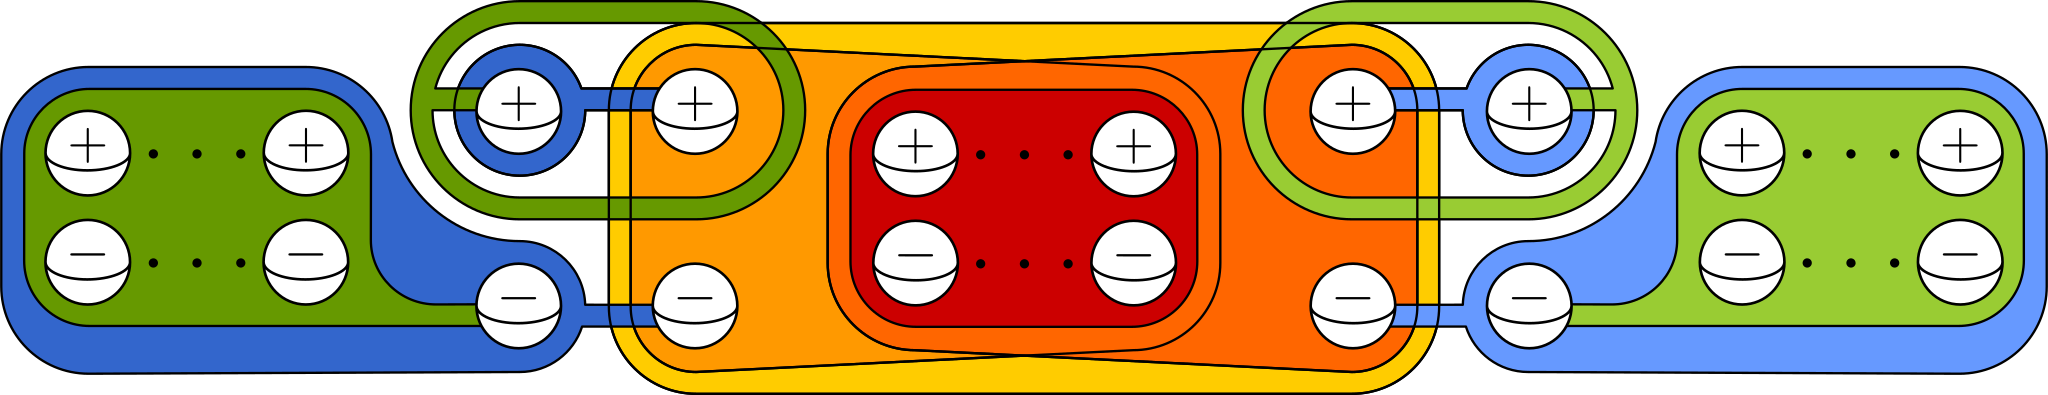
\includegraphics[width=\textwidth]{figures/ksharingnotpent.pdf}
  \caption{
    A sharing pair and the requisite carvings.
    The pair $\{x_0,x_1\}$ is shown bounding dark and light orange, respectively.
    The pair shares the $M_{k-1,1}$-bounding sphere $x$ shown bounding red.
    The pair is engulfed by $M_{k+1,1}$-bounding sphere $y$ shown in yellow.
    Dark orange $x_0$ is carved by $v_0$ and $w_0$ shown in dark green and blue.
    Light orange $x_1$ is carved by $v_1$ and $w_1$ shown in light green and blue.
  }
  \label{fig:ksharing}
  \end{figure}
\end{remark}


We call three spheres an $M_{k-1,1}$-sharing triple if
the spheres pairwise form sharing pairs and all engulf
a common $M_{k-1,1}$-bounding sphere.

\begin{lemma}
  Sharing triples are characteristic.\\
  If $\{x_0,x_1,x_2\}$ is an $M_{k-1,1}$-sharing triple with $x_0,x_1,x_2 \in \mathcal S^{sep,k}_n$
  and $\phi \in \aaut \mathcal S^{sep,k}_n$,
  then $\{\phi(x_0),\phi(x_1),\phi(x_2)\}$ is an $M_{k-1,1}$-sharing triple.
  \label{lemma:sharetrippreserve}
\end{lemma}

\begin{proof}
  According to Lemma \ref{lemma:sharepreserve}
  if $x_0,x_1,x_2$ pairwise form sharing pairs,
  then so do $\phi(x_0),\phi(x_1),\phi(x_2)$.
  It remains only to see that
  $\phi(x_0),\phi(x_1),\phi(x_2)$ all engulf a
  common $M_{k-1,1}$-bounding sphere, rather that a distinct
  $M_{k-1,1}$-bounding sphere for each pair.
  We reduce the proof to showing
  $\phi(x_0),\phi(x_1),\phi(x_2)$ all engulf a
  common $M_{k-1,1}$-bounding sphere if and only if there is
  no $M_{k+1,1}$-bounding sphere $y$ engulfing
  $\phi(x_0),\phi(x_1),$ and $\phi(x_2)$.
  Then if there were a $y$ engulfing $\phi(x_0),\phi(x_1),$ and $\phi(x_2)$, we would have
  $\phi^{-1}(y)$ engulfs $x_0,x_1,x_2$, which would contradict that
  $\{x_0,x_1,x_2\}$ is a sharing triple.

  Observe that, as in the proof of Lemma \ref{lemma:sharepreserve},
  since $\phi(x_0),\phi(x_1),\phi(x_2)$
  are pairwise sharing pairs,
  there are three pairwise-disjoint $M_{1,1}$-bounding spheres $z_0,z_1,z_2$
  such that $z_i$ is uniquely engulfed by $\phi(x_i)$ and disjoint
  but not engulfed by $\phi(x_{i+1})$, for $i \in \Z/3$.
  The sphere shared by $\{\phi(x_i),\phi(x_{i+1})\}$
  is in $\phi(x_i)^{in}-z_i^{in}$.
  If $\phi(x_0),\phi(x_1),\phi(x_2)$ all engulf a
  common $M_{k-1,1}$-bounding sphere $x$,
  then any sphere engulfing $\phi(x_0),\phi(x_1),\phi(x_2)$
  contains $x,z_0,z_1,$ and $z_2$ so must be $M_{j,1}$-bounding for $j\geq k+2$.
  If $\phi(x_0),\phi(x_1),\phi(x_2)$ do not engulf
  a common $M_{k-1,1}$-bounding sphere,
  then for $i \in \Z/3$
  we have a distinct $M_{k-1,1}$-bounding sphere
  shared by
  $\{\phi(x_i),\phi(x_{i+1})\}$ and that engulfs $z_{i-1}$.
  But then
  $\phi(x_0),\phi(x_1),\phi(x_2)$ do all engulf
  a common $M_{k-2,1}$-bounding sphere $x$
  such that $\phi(x_i)$ engulfs $x$ and $z_i$ and $z_{i+1}$.
  Then the same $M_{k+1,1}$-bounding sphere $y$ fits into the defining pentagon
  of Definition \ref{def:ksharepair}
  for all three sharing pairs.
\end{proof}

Let $x$ be an $M_{k-1,1}$-bounding sphere.
We will show that any two sharing pairs engulfing $x$
are connected by a sequence of sharing triples.
Let $\mathcal P_x$ be the \emph{sharing pair} graph defined as follows.
The vertices of $\mathcal P_x$ are $M_{k-1,1}$-sharing pairs in
$\mathcal S^{sep,k}_n$ engulfing
$x$, where $n\geq 3k$.
Two vertices $\{x_0,x_1\}$ and $\{x_1,x_2\}$
of $\mathcal P_x$ are adjacent if the pairs
have a common member and the three spheres
form an $M_{k-1,1}$-sharing triple engulfing $x$.

% By Lemma \ref{lemma:sharepreserve}, an automorphism
% $\phi \in \aaut \mathcal S^{sep,k}_n$
% induces an isomorphism
% $\mathcal P_x \stackrel{\cong}{\longrightarrow} \mathcal P_{\phi(x)}$
% .


\begin{lemma}
  The sharing pair graph $\mathcal P_x$ is connected for $n\geq 3k$ and $k\geq 2$.
  \label{lem:kshareconnect}
\end{lemma}

\begin{proof}
  We appeal to Putman's Lemma \ref{lemma:putman}.
  Fix an $M_{k-1,1}$-bounding sphere $x$ and
  an $M_{k-1,1}$-sharing pair $v=\{x_0,x_1\}$ engulfing $x$ with $x_0$ and $x_1$ having geometric intersection 1.
  Let $G \leq \oout_{n}$ be the subgroup fixing $x^{in}$, so that $G\cong \oout_{n-k+1,1}$.


  Observe that if two $x$-sharing pairs $\{x_0,x_1\}$ and $\{x_1,x_2\}$
  contain a common member $x_1$ and with all three spheres engulfed
  by a common $M_{k+1,1}$-bounding sphere $y$,
  then we can find a length 2 path in $\mathcal P_x$
  by choosing $x_3$ with intersection 1 with $y$
  and engulfing an $M_{1,1}$-bounding sphere that is disjoint from $y$.
  Then $\{x_0,x_1,x_3\}$ and $\{x_1,x_2,x_3\}$ are sharing triples, since
  they are pairwise sharing pairs and all engulf $x$.
  So if $y_0$ is the $M_{k+1,1}$-bounding sphere engulfing $v=\{x_0,x_1\}$,
  and
  $\{x'_0,x'_1\}$ is any sharing pair
  engulfed by $y'_0$,
  then there is $g \in G$ such that $g(x_1)= x'_1$ and $g(y_0) = y'_0$.
  So the orbit $G\cdot v$ is at most distance 2 from any sharing pair vertex of $\mathcal P_x$.
  This completes the first criterion of Putnam's Lemma \ref{lemma:putman}.


  Fix a system of nonseparating spheres
  $a_0, \ldots, a_{n-k}$ disjoint and not engulfed by $x$
  with $a_0$ but not $a_{n-k}$ engulfed by $x_0$ and $a_{n-k}$ but not $a_0$ engulfed by $x_1$.
  Then $G\cong \aaut \langle a_0,\ldots ,a_{n-k}, \rangle $
  is generated by diffeomorphism classes
  corresponding to
  inversions of $a_0, \ldots, a_{n-k}$ (though these always fix $v$),
  transpositions  of $a_0, \ldots, a_{n-k}$
  the transvection $t':a_0 \mapsto a_0a_1^{-1}$.

  \begin{figure}[b!]
    \centering
          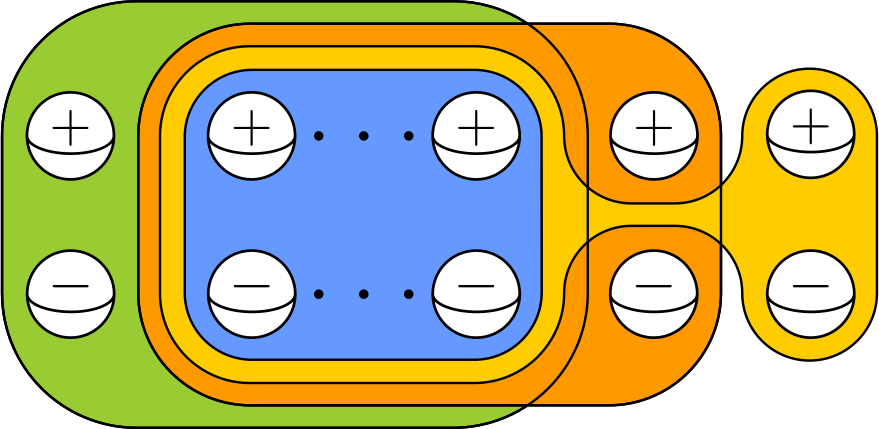
\includegraphics[width=.5\textwidth]{figures/ksharepairgraph0.pdf}
          \caption{
          The sharing pair $v$ is formed by the  green $x_1$ and  orange $x_0$ spheres.
          Transpositions move the sharing pair $v$ either distance 0 in $\mathcal P_x$,
          by swapping orange and green, or
          distance 1, by, for example, swapping orange and yellow.
          Observe that the orange, yellow, and green $M_{k,1}$-bounding spheres form a sharing
          triple for the blue sphere $x$.}
          \label{fig:ksharepair0}
  \end{figure}



  Consider first the action of   transpositions $t$ on
  the sharing pair $v \in \mathcal P_x$.
  If neither $a_0$ nor $a_{n-k}$ are swapped by $t$,
  then the sharing pair $v$ is fixed.
  If both $a_0$ and $a_{n-k}$ are swapped by $t$,
  then $x_0$ and $x_1$ are swapped, so that the sharing pair $v=\{x_0,x_1\}$
  is still fixed.
  If exactly one of $a_0$ or $a_{n-k}$ is swapped by $t$
  transposition then exactly one of $x_0$, $x_1$ are exchanged from the sharing pair,
  so that the transposition action moves the sharing pair $v$ distance 1 in $\mathcal P_x$,
  as shown in Figure \ref{fig:ksharepair0}.


  \begin{figure}[t!]
    \centering
          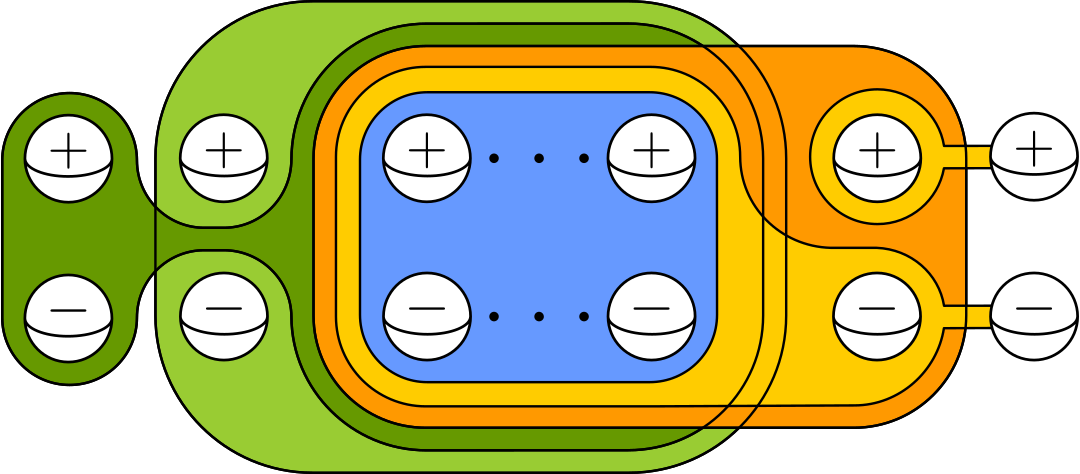
\includegraphics[width=.6\textwidth]{figures/ksharepairgraph1.pdf}
          \caption{The chosen transvection moves $v$
          distance 2 in $\mathcal P_x$.
          Observe that $x_0$ orange, $x_1$ light green,
          $x_2$ dark green, and $t'(x_0)$ yellow can be organized
          into two sharing triples: orange with the greens and yellow with the greens.}
          \label{fig:ksharepair1}
  \end{figure}

  Finally consider the transvection action $t':a_0 \mapsto a_0a_1^{-1}$ on $\mathcal P_x$.
Then $t'(x_0)$ (shown in yellow in Figure \ref{fig:ksharepair1})
intersects $x_0$ (shown in orange) twice and $t'(x_1)=x_1$ (shown in light green).
Since $n-k\geq 4$ there is a nonseparating sphere $a_2$
disjoint and not engulfed from $x_0, x_1, t'(x_0)$.
So there is an $M_{k,1}$ bounding sphere $x_2$ (shown in dark green)
engulfing $a_2$ and such that $\{t'(x_0),x_1,x_2\}$ and $\{x_0,x_1,x_2\}$ are sharing triple---
let $x_2$ be the image of $x_1$ under the transposition $(a_2a_{n-k})$.
Then we have a length 2 path of in $\mathcal P_x$
from $t'(v)$ to $v$:
$$\{t'(x_0),x_1 \} \to \{x_1,x_2\} \to \{x_0,x_1\}.$$
It follows from Putman's Lemma \ref{lemma:putman} that $\mathcal P_x$
is connected.
\end{proof}

We define a map $\aaut  \mathcal S^{sep,k}_n \to \aaut  \mathcal S^{sep,k-1}_n$
as $\phi \mapsto \hat \phi$ by extending $\phi \in \aaut  \mathcal S^{sep,k}_n$
to $M_{k-1,1}$-bounding spheres via $M_{k-1,1}$-sharing pairs.
More explicitly,
if $x \in S^{sep,k-1}_n$
is an $M_{k-1,1}$-bounding sphere
% then by Lemma \ref{lemma:ksharexist}
there is an $M_{k-1,1}$-sharing pair $\{x_0,x_1\}$
that engulfs $x$ uniquely.
Then by Lemma \ref{lemma:sharepreserve},
$\{\phi(x_0),\phi(x_1)\}$
is a sharing pair.
We define $\hat \phi (x)$ as
the $M_{k-1,1}$-bounding sphere
engulfed by $\{\phi(x_0),\phi(x_1)\}$.
By Lemma \ref{lem:kshareconnect}
any other choice $\{x'_0,x'_1\}$
of $x$-sharing pair is connected by
a sequence of sharing triples,
which by Lemma \ref{lemma:sharetrippreserve}
gives a sequence of sharing triples from
$\{\phi(x_0),\phi(x_1)\}$ to $\{\phi(x'_0), \phi(x'_1)\}$,
so that both share the same $M_{k-1,1}$-bounding sphere $\hat \phi(x)$,
which is thus well defined.

Certainly $\hat \phi$ is simplicial.
To see that observe that
if $x$ and $x'$ are disjoint
$M_{k-1,1}$-bounding spheres,
then $n \geq 3k$ so there are disjoint
$M_{k-1,1}$-sharing pairs
that $\phi$ takes to disjoint sharing pairs.
Then $\hat \phi(x)$ is disjoint from $\hat \phi(x')$.
If $y\in \mathcal S^{sep,k}_n$ is disjoint from $x$,
then $y$ is $M_{j,1}$-bounding with $j \leq \frac n 2$
so there is an $x$-sharing pair disjoint from $y$,
with its $\phi$-image disjoint from $\phi(y)$.


\begin{lemma}
  For  $n\geq 3k$ and $k\geq 2$,
  the natural restriction map
   $\aaut  \mathcal S^{sep,k-1}_n \to \aaut  \mathcal S^{sep,k}_n$
   is an isomorphism.
   \label{lemma:highsepinduct}
\end{lemma}

\begin{proof}
 We claim that the constructed map
 extension $ \aaut  \mathcal S^{sep,k}_n \to \aaut  \mathcal S^{sep,k-1}_n $
 given by $\phi \mapsto \hat \phi$
 is the inverse homomorphism to the restriction
 $ \aaut  \mathcal S^{sep,k-1}_n \to \aaut  \mathcal S^{sep,k}_n $
 with
 $\psi \mapsto \psi|_{k}$.
 By definition the restriction of $\hat \phi$ to $\mathcal S^{sep,k}_n $
 is  $\phi$.
 So the extension is injective and restriction is surjective.
 But restriction must also be injective,
 since if $\psi \in \mathcal S^{sep,k-1}_n$
 restricts to the identity,
 then for any $M_{k-1,1}$-bounding sphere $x$
 there is an $x$-sharing pair $\{x_0,x_1\}$ that $\psi$ fixes.
 But then $\psi(x)=x$ is the unique  $M_{k-1,1}$-bounding sphere
 engulfed by $\{x_0,x_1\}$.
\end{proof}


% \thmhighsep*

\begin{proof}[Proof of Theorem  \ref{thm:highsep}]
The proof is by induction on $k$ using Lemma \ref{lemma:highsepinduct}.
Theorem \ref{thm:sep} provides the base case.
\end{proof}


% \section{Coconnected Sphere Systems}
% \label{section:cocspheres}

\section{The Free Factor Complex}
\label{section:ffc}

The free factor complex $\ffn$ is the simplicial complex with a $k$-simplex given by conjugacy classes of length $k+1$ chains of proper free factors.
Bestvina and Bridson announced that the free factor complex is a combinatorial model for $\oout F_n$,
though as of this writing the result remains unpublished \cite{bridson}.


\bridson*


We proceed by proving first that the complex of coconnected spheres of $M_n$
has automorphism group $\oout F_n$.
The complex of coconnected spheres, that was introduced by Hatcher and Vogtmann to prove
homological stability results for $\oout F_n$ in \cite{homstabout},
and the complex of nonseparating spheres \cite{pandit}.
This complex is a fibration over the free factor complex.

\begin{definition}
If $F_n$ can be expressed as the internal free product of subgroups $A,B \leqslant F_n$, then $A$ and $B$ are \emph{free factors} of $F_n$.
The free factor complex has as vertices the conjugacy classes of free factors of $F_n$.
A collection of $A_1, \ldots A_k$ of free factors spans a simplex if there is
are free factors  $A'_1 < \cdots < A'_k$ such that $A_i$ is conjugate to $A'_i$.
We will frequently abuse notation and refer to both a free factor and its conjugacy class as a free factor, as dictated by context.
The distinction is rarely relevant since the free factor complex is known to be flag \cite{MR1660045}.
\end{definition}

Hatcher \cite{MR1660045} characterized the free splitting complex as a complex of spheres in $M_n$.
We define the following three simplicial complexes related to the free factor complex:
\begin{enumerate}[$\cdot$]
\item
Let $\nosep$ be the simplicial complex with $k$-simplices specified by $k+1$ disjoint nonseparating spheres in $M_n$.
\item
Let $\coc n$ be the subcomplex of $\nosep$ with simplices given by collections of spheres that are coconnected (i.e. have connected complement) in $M_n$.
\item
Let $\sfn$ be the barycentric subdivision of the $(n-2)$-skeleton of $\coc n$. Thus vertices of $\sfn$ are coconnected sets of at most $n-1$ spheres, and simplices are given by chains of proper subsets.
\end{enumerate}
For a simplex $\Sigma_0 \subset \cdots \subset \Sigma_k$ of $\sfn$, we obtain a corresponding
simplex of $\ffn$ by the (conjugacy class of) free factors $$\pi_1(M_n-\Sigma_k,x_0) \leqslant \cdots \leqslant \pi_1(M_n-\Sigma_0,x_0)$$ so we obtain a surjection of posets
$$\sfn \to (\ffn)^{op}.$$

A single nonseparating sphere of $M_n$ corresponds to a rank $n-1$ free factor of $F_n$.
The fiber over a rank $k$ free factor corresponds to all choices of collections $n-k$
factors of rank $n-1$ any $j$ of that intersect in a rank $j$ free factor.

We begin by showing

\begin{theorem}
For $n \geq 3$
the natural map
$$ \oout F_n \to \aaut{\sfn} \cong \aaut{\coc n} \cong \aaut{\nosep}$$
is an isomorphism.
\label{thm:twoisos}
\end{theorem}

The result relies on the following theorem of Pandit \cite{pandit}.

\begin{theorem}
 For $n \geq 3$ we have $\aaut{\nosep} \cong \outn$.
\end{theorem}

Our first goal is to show that $\aaut{\sfn} \cong \aaut{\coc n}$.

Let $M_{n,p}$ be the manifold $M_n$ with interiors of $p$ disjoint closed  balls removed. We call $n$ the \emph{genus} of $M_{n,p}$. If $\Sigma$ is a set of disjoint embedded spheres of $M_{n,p}$, we will denote by $M_{n,p}|\Sigma$ the manifold $M_{n,p}$ cut along $\Sigma$.

\begin{lemma}
Automorphisms of $\sfn$ preserve the cardinality of sets of spheres.
\label{lemma:samenumspheres}
\end{lemma}

\begin{proof}
We induct downward on the cardinality of sets of spheres.
We claim as a base case that a set of spheres $\Sigma \in \sfno$ has $n-1$ spheres if and only if
it is adjacent to finitely many sets of spheres in $\sfn$, namely, the proper subsets of $\Sigma$.
If $\Sigma \in \sfno$ has fewer than $n-1$ spheres, then
$M_n|\Sigma$ has genus $k \geq 2$.
The complex of coconnected nonseparating spheres of $M_n|\Sigma$ is isomorphic to $\coc k$, which is infinite.
Choose any nonseparating sphere $a$ of $M_n|\Sigma$. Then $\Sigma \cup \{a\}$ is coconnected in $M_n$ and adjacent to $\Sigma$ in $\sfn$.

Assume that automorphisms of $\sfn$ preserve the size of sets of spheres with at least $k+1$ spheres.
Let $A_k \subset \sfno$ be the sets of spheres of $\sfn$ with $k$ or fewer spheres.
A set of spheres $\Sigma \in A_k$ has $k$ spheres if and only if $\link(\Sigma) \cap A_k$ is finite.
By hypothesis automorphisms of $\sfn$ preserve $A_k$ and its complement, so must preserve the class of sets of $k$ spheres.
\end{proof}

We now prove the first isomorphism of Theorem \ref{thm:twoisos}.\\

\begin{lemma}
For $n\geq 3$ we have $\aaut \sfn \cong \aaut{\coc n}$.
\end{lemma}

\begin{proof}
As $\sfn$ is the barycentric subdivision of the $n-2$ skeleton ${\coc n}^{(n-2)}$, there is a natural map
$$\Phi: \aaut{\coc n} \to \aaut{\sfn}.$$ We will construct the inverse. Let $\phi \in \aaut{\sfn}$.
The vertices of $\sfn$ are the simplices of $\coc n$ with dimension $n-2$ or less.
Then $\phi$ induces a bijection $\phi_\ast$ of simplices of ${\coc n}^{(n-2)}$.
By Lemma \ref{lemma:samenumspheres} we have $\phi_\ast$ preserves the dimension of simplices, so $\phi_\ast$ is an automorphism of ${\coc n}^{(n-2)}$.

It remains to see that $\phi_\ast$ also preserves $n-1$ simplices.
To see this we will show that a collection of $n$ disjoint separating spheres $\Sigma$ form a simplex in $\coc n$ if and only if
$$\coc n \cap  \left ( \bigcap_{x \in \Sigma} \link(x) \right )$$
is finite.
Note that if $\Sigma$ is a coconnected set of $n$ spheres, then $M_n|\Sigma$ is homeomorphic to $M_{0,2n}$. Then $\pi_2(M_n|\Sigma)$ is the free abelian group generated by any $2n-1$ of the balls, and an embedded sphere must be degree at most 1 over any generator.
There are thus finitely many  embedded spheres of $M_n|\Sigma$.
Then $\bigcap_{x \in \Sigma} \link (x)$ contains finitely many vertices of $\coc n$.
Conversely suppose $\Sigma$ is a non-coconnected set of $n$ disjoint spheres.
Then $M_n|\Sigma$ has a component $M'$ with genus at least one and at least two boundary spheres.
Choose a nonseparating sphere $x$ of $M'$, a boundary sphere $y$, and a loop $\alpha$ based at $y$ intersecting $x$ once. The push map of $x$ along $\alpha$ produces a collection $A$ of infinitely many spheres of $M_n$. Each $a \in A$ is nonseparating in $M' \subset M|\Sigma$, so $\{a,x\}$ is coconnected for any $x \in \Sigma$. Then  $A\subset \bigcap_{x \in \Sigma} \link (x)$.
Thus $\phi_\ast$ must also preserve $n-1$ simplices and gives a simplicial automorphism of $\coc n$.
Then $\phi \mapsto \phi_\ast$ gives the inverse homomorphism to $\Phi$.
\end{proof}



Call a collection of $m$ disjoint spheres $\Sigma \subset {\coc n}^{(0)}$ a \emph{bounding $m$-tuple} (pair, triple, etc.) if $\Sigma$ is not coconnected but every proper subset of $\Sigma$ is.
The genus of the bounding tuple is the smaller of the genera of the two components of $M_n|\Sigma$.
The following lemma shows we can detect the genus combinatorially.

\begin{lemma}
The link of a genus $k$ bounding $m$-tuple of $\coc n$ is isomorphic to the join $\coc{k} \ast \coc{n-k-m+1}$.
\label{lemma:itwasseven}
\end{lemma}

\begin{proof}
Consider $\Sigma \subset {\coc n}^{(0)}$ a bounding $m$-tuple with genus $k$.
Then $M_n|\Sigma$ has two components, $R_1 \cong M_{k,m}$ and $R_2 \cong M_{n-k-m+1,m}$.
Let $V_i$ be the complex of coconnected nonseparating spheres in $R_i$.
So $V_1 \cong {\coc {k}}$ and $V_2 \cong \coc {n-k-m+1}$.
We claim that $\link(\Sigma)$ is the join $V_1 \ast V_2$.
Certainly $\link(\Sigma) \subset V_1 \ast V_2$.
Consider sets of spheres $\Sigma_i$ giving simplices of $V_i$.
The $R_i|\Sigma_i$ are connected. $M_n|(\Sigma_1 \cup \Sigma_2)$ is $R_1|\Sigma_1$ and $R_2|\Sigma_2$ glued along $\Sigma$, and hence connected. So $\Sigma_1\cup \Sigma_2$ must be coconnected in $M_n$ and the join $\Sigma_1 \ast \Sigma_2$ lies in $\link(\Sigma)$.
\end{proof}

We now prove the second isomorphism of Theorem \ref{thm:twoisos}.\\

\begin{lemma}
  For $n\geq 3$ we have $\aaut{\coc n} \cong \aaut{\nosep}$.
\end{lemma}

\begin{proof}
Restriction gives a natural map
$$\Phi: \aaut{\nosep} \to \aaut{\coc n}.$$
We will construct the inverse.
Observe that since ${\coc n}^{(0)} = {\nosep}^{(0)}$ any $\phi \in \aaut{\coc n}$ induces a set map $\phi_\ast$ of ${\nosep}^{(0)}$.
If $\phi_\ast$ is a simplicial automorphism, then $\phi \mapsto \phi_\ast$ is the inverse homomorphism to $\Phi$.
As $\nosep$ is a flag complex (Lemma 3 of \cite{souto}), it will suffice to show that $\phi_\ast$ sends pairs of disjoint spheres to pairs of disjoint spheres.
Disjoint nonseparating spheres form a bounding pair if and only if they are not adjacent in $\coc n$.
So it suffices to show that $\phi$ preserves bounding pairs of $\coc n$.
We will demonstrate this through the stronger result that $\phi$ preserves the set of genus $k$ bounding $m$-tuples.

\emph{Case 1.} Suppose $\Sigma$ is a genus $k$ bounding $m$-tuple with $m>2$. Any $\Sigma' \subset {\coc n}^{(0)}$ is a bounding $m$-tuple if and only if $\Sigma'$ does not span a simplex in $\coc n$, but every proper subset of $\Sigma'$ does. Hence if $\phi \in \aaut{\coc n }$, then $\phi(\Sigma)$ is a bounding $m$-tuple.
By Lemma \ref{lemma:itwasseven}, $\link(\Sigma)$ is isomorphic to $\coc {k} \ast \coc{n-k-m+1}$. We can determine $k$ by the maximal simplex dimension on the sides of the join. Then $\phi(\Sigma)$ is also genus $k$.

\begin{figure}[b!]
\includegraphics[width=\textwidth]{figures/spheresagain.pdf}
\caption{
The manifold $M_n|\{a_i\}_{i=1}^n$ is a 3-sphere with $2n$ balls removed.
We obtain $M_n$ by again identifying the spheres with $+$ and $-$ labels via a vertical reflection.
The spheres $\Sigma'=\{x_i,y_i\}_{i=1}^4$ are such that $M_n|\Sigma'$ contains $x$ and $y$ in disjoint copies of $M_{0,4}$. The $M_{0,4}$ containing $x$ (identify $x^+$ and $x^-$) is shaded. The $M_{0,4}$ containing $y$ is the exterior of $y_2$ and $y_3$.
}
\label{fig:spherediagram}
\end{figure}

\medskip \noindent \emph{Case 2.} Suppose $\Sigma=\{x,y\}$ has $m=2$ spheres.
Choose a collection $\Sigma'$ of disjoint nonseparating spheres such that  there are two separate components of $M_n|\Sigma'$ homeomorphic to $M_{0,4}$ and containing $x$ and $y$ respectively.
We can construct $\Sigma'$ as follows.
$M_n|\Sigma$ has two components, homeomorphic to $M_{k,2}$ and $M_{n-k-1,2}$.
So we have a set of spheres $\{a_i\}_{i=1}^n$ coconnected in $M_n$ disjoint from $y$ with $a_{k+1}=x$.
Choose $x_2,x_3,y_2,y_3$ as shown in figure \ref{fig:spherediagram} and relabel $a_1=y_1$, $x_{1}=a_k$, $x_4=a_{k+2}$, $y_4=a_n$.
Then
$\{x_1,\ldots, x_4\}$ (resp. $\{y_1, \ldots, y_4\}$ are the boundary spheres of a component of $M|\Sigma'$ homeomorphic to $M_{0,4}$ and containing $x$ (resp. $y$).
Further $\{x,x_1,x_2\}$ and $\{x,x_3,x_4\}$ are genus 0 bounding triples. Let $\Sigma' =\{x_i,y_i\}_{i=1}^4$.



By Case 1 we have that $\{\phi(x_1), \ldots, \phi(x_4)\}$ is a genus 0 bounding $4$-tuple and $\{\phi(x),\phi(x_1),\phi(x_2)\}$ and $\{\phi(x),\phi(x_3),\phi(x_4)\}$ are genus 0 bounding triples.
So $\{\phi(x_1), \ldots, \phi(x_4)\}$ define a component of $M|\Sigma'$ homeomorphic to $M_{0,4}$ and containing $\phi(x)$.

If $\{x_1, \ldots, x_4\} \neq \{y_1, \ldots, y_4\}$ then
 $\phi(x)$ and $\phi(y)$ lie in disjoint $M_{0,4}$ homeomorphic components of $M|\phi(\Sigma')$.
Then  $\phi(x)$ and $\phi(y)$ are are disjoint. They are also not adjacent in $\coc n$, so they are bounding a pair.

Suppose $\{x_1, \ldots, x_4\} = \{y_1, \ldots, y_4\}$.
Then $n=3$ and $M_3|\{x_i\}_{i=1}^4$ is homeomorphic to two copies of $M_{0,4}$.
As $x,y$ form a bounding pair, the bounding triples must be
$\{x,x_1,x_2\}$, $\{x,x_3,x_4\}$, $\{y,x_1,x_2\}$, and $\{y,x_3,x_4\}$.
Then the $\phi$ image of these triples are
bounding triples giving $\phi(x)$ and $\phi(y)$ contained in disjoint $M_{0,4}$.
Then $\phi(x)$ and $\phi(y)$ are disjoint and must form a bounding pair.
\end{proof}


% \section{Complex of Surfaces}
%
% \noindent \emph{Def}
% A genus $g$ \emph{rosebud} is the wedge of a sphere and a genus $g$ rose.
% We consider spheres genus 0 rosebuds, and roses degenerate rosebuds.\\
% \\
%
% \noindent \emph{Claim}
% Every embedded compact
% closed orientable surface in $M_g$
% is homotopy equivalent to a sphere, rose, or rosebud.\\
% \\
% \emph{Proof.}
% Consider the image in $p^3$ minus spheres.
% Every disk is compressible.\qed\\
% \\
%
% \noindent \emph{Claim}
% An embedded surface $p_g$ has $\pi_1(S_g)$ contains a
% free factor at most rank $g$.\\
% \\
% \emph{Proof.}
% If $\pi_1(S \hookrightarrow M)$ contains a free factor rank $k$,
% then $p$ intersects at least $k$ disjoint spheres
% in $M$. Then there are at least $k$
% compressible disks with $\partial D \subset S$.
% Each one kills a generator of $\pi_1(S)$
% \\
%
% \noindent \emph{Claim}
% There is a correspondence between
% homotopy classes of embedded rosebuds
% in $M_n$ and one edge Bass Serre graph-of-groups
% decompositions of $F_n$.\\
% \\
% \emph{Proof.}
% By Van Kampen every rosebud gives a graph of groups.
% Conversely if $F_n =  \pi_1 ( A \leftrightarrow C \rightarrow B )$
% then there is a basis $\{a_i\}_{i \in n}$ of $F_n$
% with the first $k$ in $A$ and the last $n-k$ in B.
% This corresponds to a system of nonseparating spheres.
% There is a unique separating sphere $p$ which separates the $A$
% spheres from the $B$ spheres.
% From a basepoint on $p$ there is a rose whose petals give the arcs forming
% a basis of $C$. \qed\\
% \\
%
% \noindent \emph{Def. }
% The graph of embedded rosebuds
% $\mathcal R_n$
% has embeddings of rosebuds (and roses) of genus at most $n$ as vertices.
% Two embedded rosebuds are adjacent if the embeddings of their
% homotopy classes differ by
% the wedge of a (homologically nontrivial?) 1- or 2-sphere.\\
%
%
% 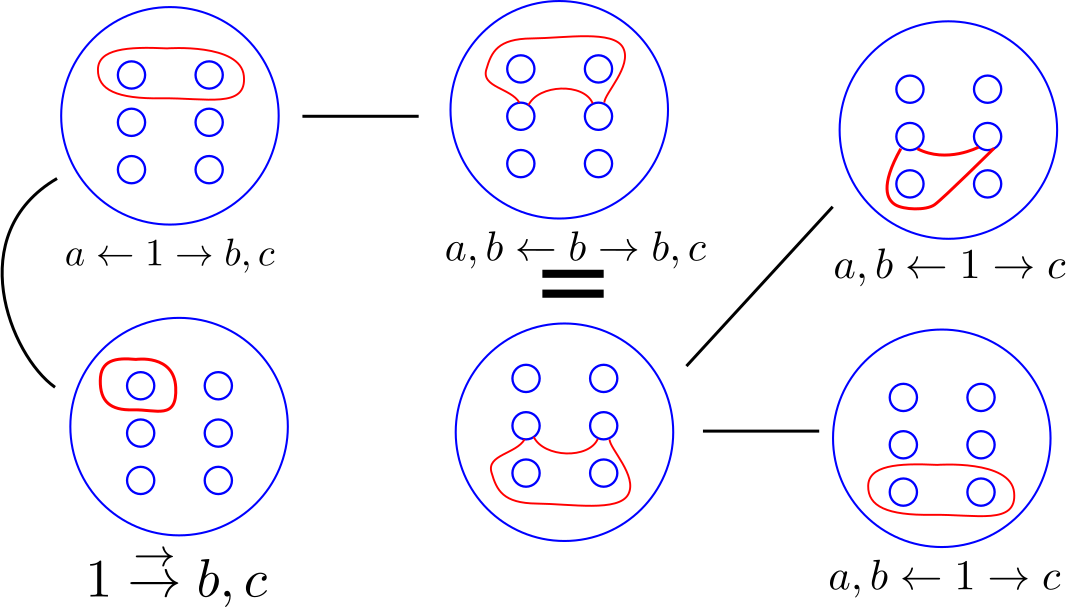
\includegraphics[width=.8\textwidth]{figures/rosebudgraph.pdf}
%
%
% $\mathcal R_n$ is equivalent to the graph of one-edge Bass Serre
% graph-of-group decompositions of $F_n$ with adjacency given by
% the following moves:
% \begin{enumerate}
%   \item tube tunneling at $a \in A - B$
%   $$A \leftarrow C \rightarrow B  \ \Leftrightarrow  \ A \leftarrow C \ast a \rightarrow B \ast a$$
%   \item nonseparating sphere scooping (primitive $b \not \in A$)
%   $$
%    C \stackrel{\rightarrow}{\rightarrow} A \ast A'b
%     \ \Leftrightarrow  \
%     C \stackrel{\rightarrow}{\rightarrow}  A \ast A'
%      \ \Leftrightarrow  \
%   b \ast C \leftarrow C \rightarrow  A \ast A'
%   $$
% \end{enumerate}



Dyer and Formanek gave an algebraic proof
of the fact that automorphisms of automorphisms of free groups are simply automorphisms of free groups \cite{doi:10.1112/jlms/s2-11.2.181}.
Vogtmann and Bridson gave a more recent geometric proof \cite{MR1769698}.
\begin{theorem}
  The natural maps
  $$\aaut F_n \to \aaut \aaut F_n$$
  and
  $$\oout F_n \to \aaut \oout F_n$$
  are isomorphisms for $n \geq 3$.
  In particular $\oout \oout F_n =1$ and the center of $\oout F_n$ is trivial.
  \label{theorem:outout}
\end{theorem}


\begin{lemma} Automorphisms of the free factor complex preserve the rank of free factors.

  Let $\phi \in \aaut \ffn$ and let $A$ be a free factor of $F_n$.
  Then $A$ and $\phi(A)$ have the same rank.
  \label{lemma:ffsize}
\end{lemma}

\begin{proof}
  Suppose that $A$ is a free factor of $\ffn$.
  Then the link of $A$ is a join
  $$
  \link A \cong  \mbox{span} \{B \in \ffn^{(0)} \ | \ B < A\} \ast \mbox{span} \{B \in \ffn^{(0)}  \ | \ A<B\}
  $$
  between the sub- and  super-factors of $A$.
  So if $A$ is rank $k$ then
  $\{B \in \ffn^{(0)} \ | \ B < A\}$ spans a dimension $k-2$ subcomplex
  isomorphic to $\mathcal{FF}_k$ and similarly $\{B \in \ffn^{(0)}  \ | \ A<B\}$
  spans a dimension $n-k-2$ subcomplex
  isomorphic to $\mathcal{FF}_{n-k}$.
  If $\phi \in \aaut \ffn$ then $\phi$ preserves this join and $\phi(A)$ must be either rank $k$ or $n-k$.

  Let $\mathcal G$ be the subcomplex of $\ffn$ spanned by rank 1 and rank $n-1$ free factors.
  Then $\mathcal G$ is a connected and bipartite with the rank 1 and rank $n-1$ factors forming the parts of the bipartition.
  Then if $A,A' \in \mathcal G^{(0)}$ are free factors the same rank, the free factors $\phi(A),\phi(A')$ must have the same rank for any $\phi \in \aaut \ffn$.
  Assume to the contrary that there is $\phi \in \aaut \ffn$ an automorphism
  and a rank $n-1$ free factor $A$ with $\phi(A)$ rank 1.
  Then $\phi$ must swap the bipartition of $\mathcal G$.
  In fact, there is a map $\aaut \ffn \to \Z/2$ taken by sending $\phi' \in \aaut \ffn$ to the generator of $\Z/2$
  if $\phi'$ swaps the bipartition on $\mathcal G$.
  Then if $G = \langle \phi, \oout F_n \rangle  \leq \aaut \ffn$ is the subgroup generated by $\oout F_n$ and the automorphism $\phi$
  we have an exact sequence
  $$
  \begin{tikzcd}
    1 \arrow{r} &
    \oout F_n \arrow{r} &
    G  \arrow{r}&
    \Z/2  \arrow{r}&
    1
  \end{tikzcd}
  $$
  But by Theorem \ref{theorem:outout} we know $\oout F_n$ is centerless and $\oout \oout F_n = 1$,
  so we may apply Lemma
  \ref{centerout}
  to conclude that $G \cong \oout F_n  \times \Z/2$.
  Then there is an order two automorphism $t$ of $\ffn$ that swaps the bipartition of $\mathcal G$
  and commutes with $\oout F_n$.
  Then there is rank one free factor $\langle b \rangle$ and free factor $A$ with rank $n-1$
  such that $t(\langle b \rangle )=A$.
  Let $A$ have free basis $a_1,\ldots,a_{n-1}$ with $b=a_{n-2}$ if $b \in A$.
  Then the transvection $\phi''$ with $b \mapsto ba_1$ and $a_i \mapsto a_i$
  is an outer automorphism acting on the free factors with
  $$
  A = \phi''(A) =\phi'' t(\langle b \rangle ) = t \phi'' ( \langle b \rangle ) = t ( \langle ba_1 \rangle  )
  $$
  but this contradicts that $t$ is injective.
  It must be that for any automorphism $\phi \in \ffn$
  the rank of $A$ and $\phi(A)$ are the same if $A$ is rank 1 or rank $n-1$.

  But then if $A$ is a rank $k$ free factor, the link of $A$ is a join with sides of dimension $k-2$ and $n-k-2$,
  and any rank $n-1$ free factor $B$ containing $A$ is on the dimension  $n-k-2$ side.
  So the link of $\phi(A)$  is isomorphic to $\mathcal{FF}_k \ast \mathcal{FF}_{n-k}$
  with $\phi(B)$ the rank $n-1$ free factor on the dimension $n-k-2$ side.
  But then $\phi(A)$ must be rank $k$ as well.
\end{proof}


% \begin{theorem}
%   The natural map
%   $$
%   \oout F_n \to \mathcal{FF}_n
%   $$
%   is an ismorphism for $n \geq 3$.
%   \label{}
% \end{theorem}

\bridson*

\begin{proof}
  Let $A$ be a free factor of rank $n-1$.
  Recall the bijection between the conjugacy classes of rank $n-1$ free factors and homotopy classes of nonseparating spheres of $M_n$.
  There is a unique nonseparating sphere $z$ in $M_n$
  specifying the conjugacy class of a free factor $A_x$ in $\pi_1 (M_n-x,q)$.
  So if $\phi \in \aaut \ffn$ we define a map of spheres by defining $\hat \phi(x)$ to be the sphere
  specifying the free factor $\phi(A_x)$ for any nonseparating sphere $x$.
  If $\Sigma$ is a coconnected set of $k$ spheres
  then we have the conjugacy class representatives of free factors $A_x$ for $x\in \Sigma$ such that $\bigcap_{x \in \Sigma'} A_{x'}$
  is a free factor of rank $n-|\Sigma'|$ for any $\Sigma' \subset \Sigma$.
  Coversely, if $A_1, \ldots, A_\ell$ are rank $n-1$ free factors bijecting to nonseparating spheres $x_1, \ldots, x_\ell$
  such that $\bigcap_{j \in s} A_j$ a rank $n-|s|$ free factor for any $s \subset \{1, \ldots, \ell\}$ then it must be that
  $$F_n  = \bigcap_{j=1}^\ell A_j \ast \langle a_1 \rangle  \ast \cdots \ast \langle a_\ell \rangle$$
  for some $a_j \in A_j$ so that $\{x_j\}_{j=1}^\ell$ must be coconnected nonseparating spheres.

  Then by Lemma \ref{lemma:ffsize} this property is preserved by $\phi$, so that
  we have a well defined simplicial map $\hat \phi: \sfn \to \sfn$
  with
  $\hat \phi (\Sigma) = \{ \hat \phi(x) \ | \ x \in \Sigma \}$.
  This gives us homomorphisms
  $$
  \begin{tikzcd}
    \oout F_n \arrow[hookrightarrow]{r} &
    \aaut \ffn \arrow{r}{\hat{\cdot}} &
    \aaut \sfn\\
    &
    \phi \arrow[mapsto]{r} & \hat \phi
  \end{tikzcd}
  $$
If $\hat \phi$ fixes every coconnected set of sphere then $\phi$ must fix every free factor,
so these homomorphisms are in fact isomorphisms.
\end{proof}
